\clearpage
\subsection{実習3-4 力センサの電圧電流特性}
\begin{itemize}
	\item プログラムは上記の\ref{ex32-block}と同じものを利用し,$R_{0}$の値は10\,k\rm{$\Omega$}とした.
	\item 計測結果は\wtab{PS}のようになった.
	\item 計測データを基に作成した電圧電流特性のグラフは\wfig{3-4}である.
\end{itemize}

\begin{table}[h]
  \centering
    \caption{力センサの諸特性値}
    \label{tab:PS}
     \scalebox{0.8}{
    \begin{tabular}{ccccc}
    \hline
    カウンタ変数 & 自然状態での$V_{U}$[\rm{V}] & 自然状態での$I_{U}$[\rm{A}]  & 圧力ありでの$V_{U}$[\rm{V}] &圧力ありでの$I_{U}$[\rm{A}] \\
    \hline
 0  & 0.007324 & 0.0000001  & 0.006104 & 0.000000122 \\
1  & 0.100098 & -0.0000001 & 0.019531 & 0.00000793 \\
2  & 0.198975 & 0.0000000  & 0.037842 & 0.0000157 \\
3  & 0.299072 & -0.0000002 & 0.058594 & 0.0000237 \\
4  & 0.397949 & -0.0000001 & 0.081787 & 0.0000316 \\
5  & 0.494385 & 0.0000005  & 0.102539 & 0.0000397 \\
6  & 0.593262 & 0.0000004  & 0.12085  & 0.0000477 \\
7  & 0.692139 & 0.0000005  & 0.136719 & 0.0000559 \\
8  & 0.789795 & 0.0000007  & 0.161133 & 0.0000636 \\
9  & 0.887451 & 0.0000011  & 0.177002 & 0.0000720 \\
10 & 0.987549 & 0.0000010  & 0.194092 & 0.0000804 \\
11 & 1.086426 & 0.0000011  & 0.218506 & 0.0000880 \\
12 & 1.185303 & 0.0000012  & 0.236816 & 0.0000959 \\
13 & 1.28418  & 0.0000015  & 0.253906 & 0.000104 \\
14 & 1.381836 & 0.0000015  & 0.269775 & 0.000113 \\
15 & 1.483154 & 0.0000016  & 0.289307 & 0.000121 \\
16 & 1.58081  & 0.0000017  & 0.307617 & 0.000129 \\
17 & 1.678467 & 0.0000020  & 0.323486 & 0.000137 \\
18 & 1.779785 & 0.0000020  & 0.343018 & 0.000146 \\
19 & 1.876221 & 0.0000022  & 0.357666 & 0.000154 \\
20 & 1.975097 & 0.0000022  & 0.371094 & 0.000163 \\
21 & 2.075195 & 0.0000022  & 0.396728 & 0.00017  \\
22 & 2.172851 & 0.0000026  & 0.411377 & 0.000179 \\
23 & 2.272949 & 0.0000026  & 0.428467 & 0.000187 \\
24 & 2.370605 & 0.0000027  & 0.445557 & 0.000195 \\
25 & 2.470703 & 0.0000028  & 0.461426 & 0.000204 \\
26 & 2.568359 & 0.0000031  & 0.482178 & 0.000212 \\
27 & 2.667236 & 0.0000033  & 0.496826 & 0.00022  \\
28 & 2.766113 & 0.0000033  & 0.511475 & 0.000229 \\
29 & 2.86499  & 0.0000035  & 0.531006 & 0.000237 \\
30 & 2.963867 & 0.0000035  & 0.540771 & 0.000246 \\
31 & 3.063965 & 0.0000035  & 0.552978 & 0.000255 \\
32 & 3.161621 & 0.0000038  & 0.562744 & 0.000263 \\
33 & 3.261718 & 0.0000038  & 0.579834 & 0.000272 \\
34 & 3.360595 & 0.0000039  & 0.5896   & 0.000281 \\
35 & 3.459472 & 0.0000042  & 0.609131 & 0.000289 \\
36 & 3.558349 & 0.0000042  & 0.625    & 0.000297 \\
37 & 3.658447 & 0.0000042  & 0.635986 & 0.000306 \\
38 & 3.757324 & 0.0000045  & 0.653076 & 0.000314 \\
39 & 3.85498  & 0.0000046  & 0.664062 & 0.000324 \\
40 & 3.953857 & 0.0000046  & 0.679932 & 0.000332 \\
41 & 4.053955 & 0.0000045  & 0.690918 & 0.000341 \\
42 & 4.152832 & 0.0000048  & 0.716553 & 0.000348 \\
43 & 4.252929 & 0.0000049  & 0.725098 & 0.000358 \\
44 & 4.348144 & 0.0000051  & 0.738525 & 0.000366 \\
45 & 4.449462 & 0.0000050  & 0.756836 & 0.000374 \\
46 & 4.547119 & 0.0000055  & 0.770264 & 0.000383 \\
47 & 4.644775 & 0.0000057  & 0.793457 & 0.000391 \\
48 & 4.744873 & 0.0000056  & 0.814209 & 0.000398 \\
49 & 4.846191 & 0.0000054  & 0.837402 & 0.000406 \\
50 & 4.942626 & 0.0000056  & 0.863037 & 0.000414 \\
\hline
\end{tabular}
}
\end{table}

\begin{figure}[h]
\centering
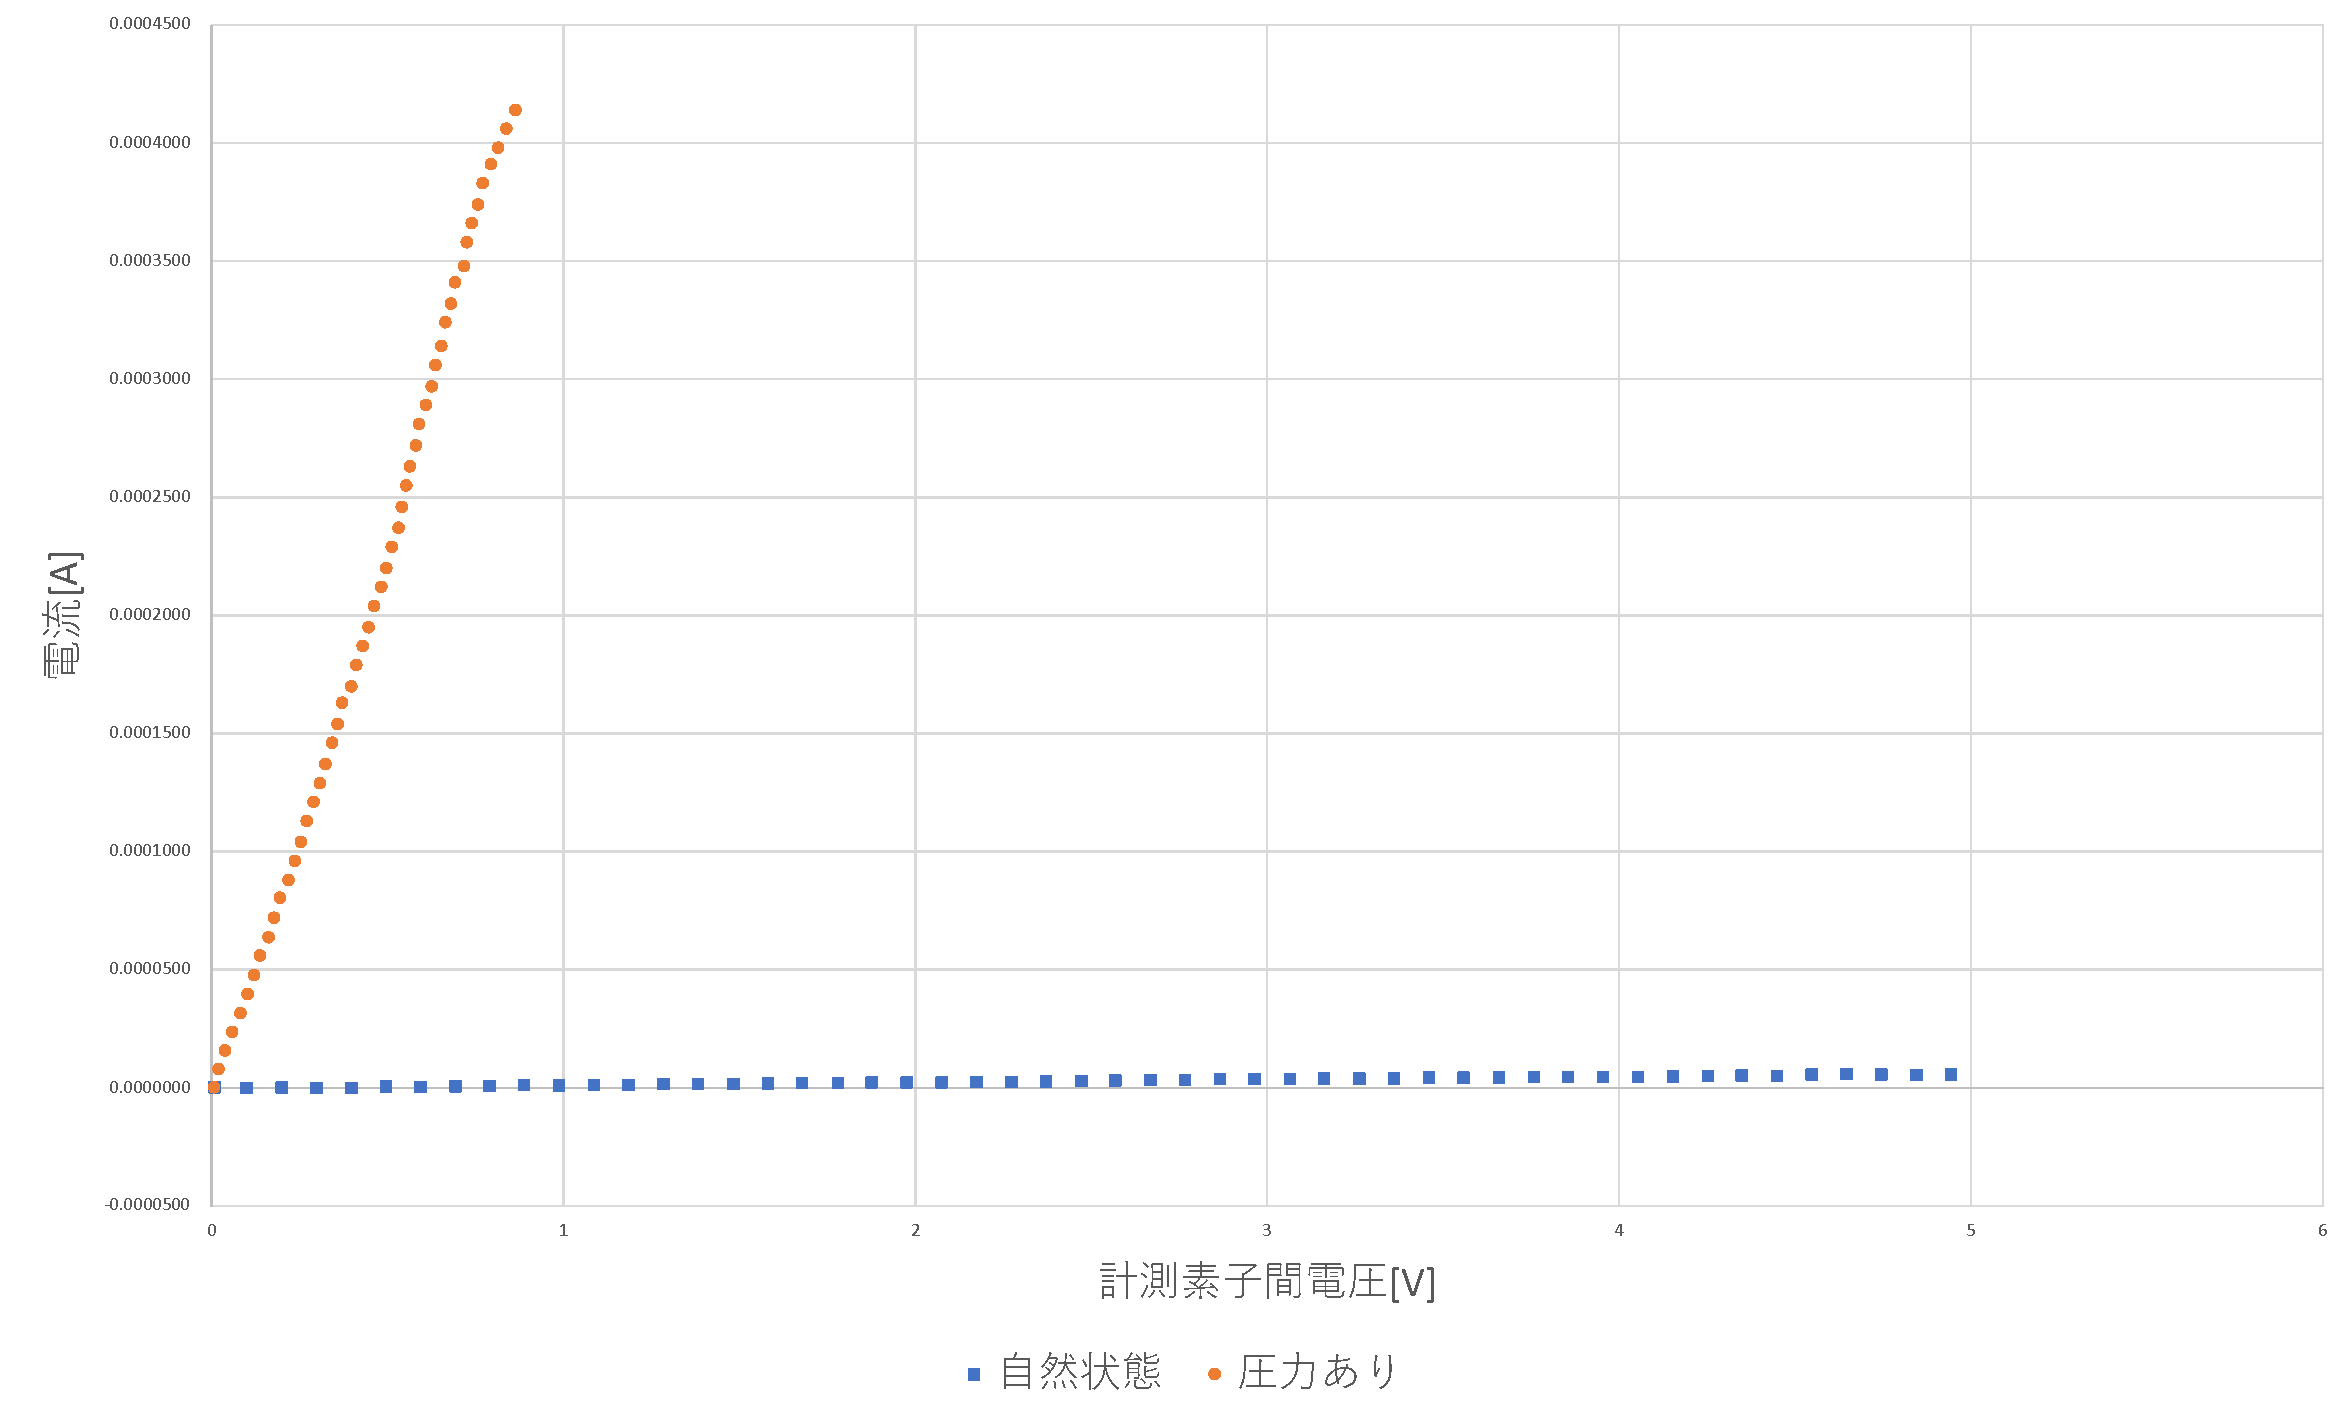
\includegraphics[scale=0.45]{./fig/3-4.pdf}
\caption{力センサの電圧電流特性}
\label{fig:3-4}
\end{figure}